\documentclass{article}
\usepackage{listings}
\usepackage{graphicx}
\usepackage{float}



\begin{document}

\centerline{\sc \large CS 558: Quiz 5}
\vspace{.5pc}
\centerline{Alana Laryssa Seabra A Santos}
\centerline{\it 3/2/2016}
\vspace{1pc}

\section{First problem}

Here are three images for problem 1:

\begin{figure}[h]
\centering
  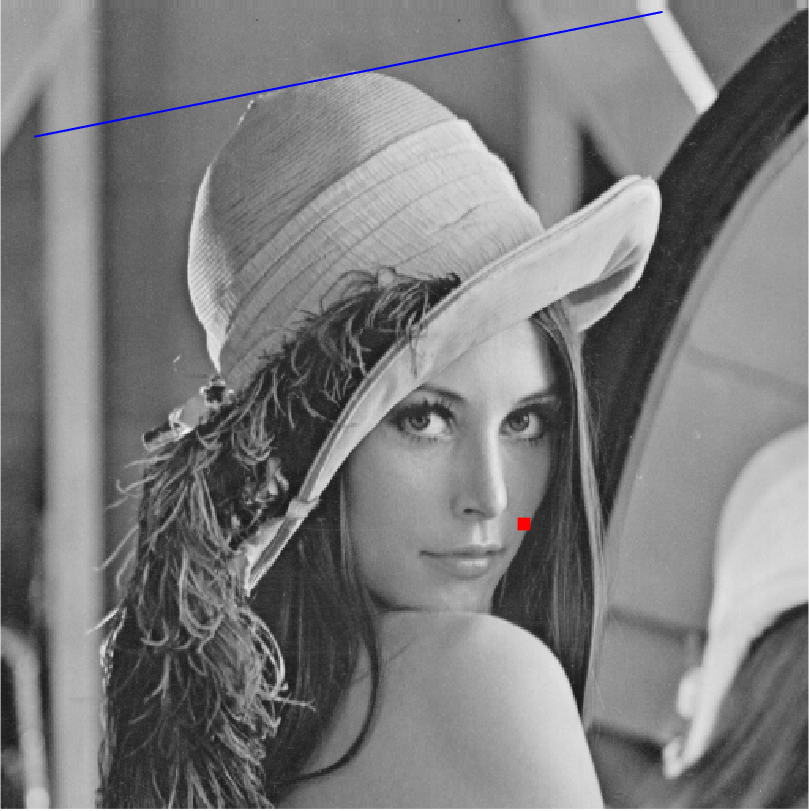
\includegraphics[scale=0.45]{../prob1.png}
\end{figure}

\begin{figure}[h]
\centering
  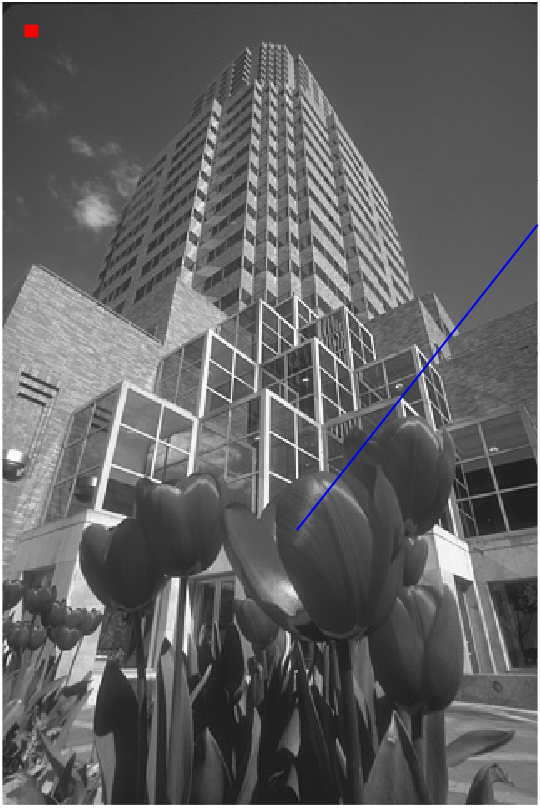
\includegraphics[scale=0.5]{../prob1a.png}
\end{figure}

\begin{figure}[h]
\centering
  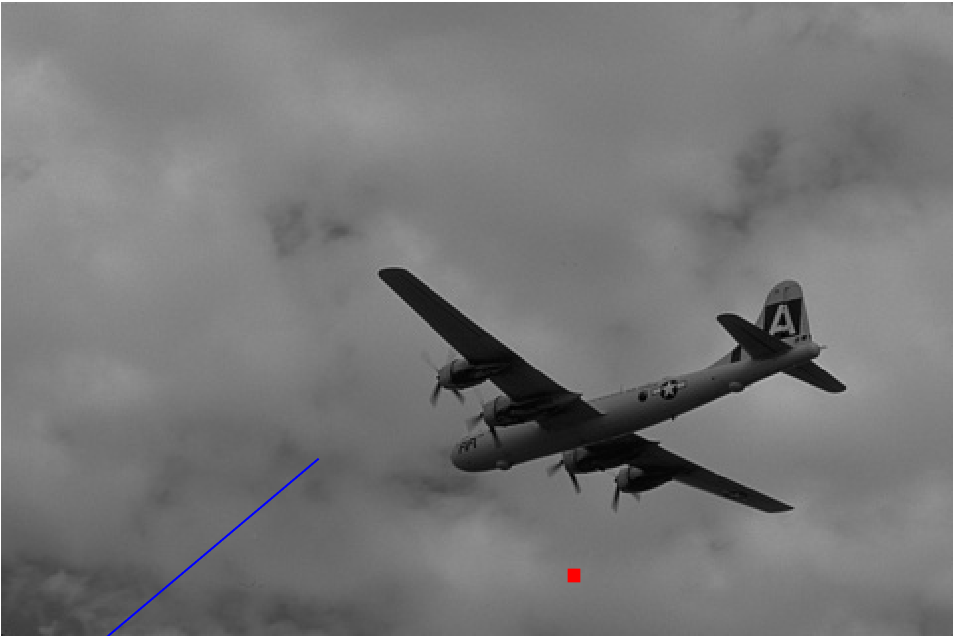
\includegraphics[scale=0.5]{../prob1b.png}
\end{figure}


\subsection{Matlab code}
\begin{lstlisting}[language=Matlab]

im = rgb2gray(imread('lena.png'));
[s1,s2] = size(im);
h1 = imshow(im);

% blue line
p1x = round(rand(1)*s1); p1y = round(rand(1)*s2);
p2x = round(rand(1)*s1); p2y = round(rand(1)*s2);

hold on;
lin = line([p1x p2x], [p1y p2y], 'Color', 'b', 'LineWidth', 1.5);

% red square
p3x = round(rand(1)*s1); p3y = round(rand(1)*s2);
halfwin = 1;

[xx,yy] = meshgrid(p3x-halfwin:p3x+halfwin, p3x-halfwin:p3x+halfwin);
hold on;
sq = scatter(xx(:),yy(:),'filled','square','r');


\end{lstlisting}

\vspace{1pc}
\section{Second problem}

The line format is $ax + by = d$, with $a^2 + b^2 = 1$. So I selected $b$ in terms of $a$, instead of dividing the distance equation by the norm of the vector $(a,b)$.
\\
\\
\\
\subsection{Matlab code}
\begin{lstlisting}[language=Matlab]
p0x = rand(1); p0y = rand(1);
a = rand(1);
b = sqrt(1 - a.*a);
d = rand(1);

dist = abs(a*p0x + b*p0y - d);
\end{lstlisting}

\vspace{1pc}
\section{Third problem}

Here, I used the fact that both points $P_1 = (x_1,y_1)$ and $P_2 = (x_2,y_2)$ lie on the line, so $\rho = x_1\cos{\theta} + y_1\sin{\theta}$ and  $\rho = x_2\cos{\theta} + y_2\sin{\theta}$. Then, $(x_1 - x_2)\cos{\theta} = (y_2 - y_1)\sin{\theta}$, and finally $\tan{\theta} = \frac{x_1-x_2}{y_2-y_1}$. To find $\rho$, we just need to plug $\theta$ in one of the equations.

\subsection{Matlab code}
\begin{lstlisting}[language=Matlab]
p1x = rand(1)*100; p1y = rand(1)*100;
p2x = rand(1)*100; p2y = rand(1)*100;

th = atan((p1x-p2x)/(p2y-p1y));
rho = p1x*cos(th) + p1y*sin(th);
\end{lstlisting}


\end{document}


